%%%%%%%% ICML 2026 EXAMPLE LATEX SUBMISSION FILE %%%%%%%%%%%%%%%%%

\documentclass{article}

% Recommended, but optional, packages for figures and better typesetting:
\usepackage{microtype}
\usepackage{graphicx}
\usepackage{subcaption}
\usepackage{booktabs} % for professional tables
\usepackage[dvipsnames]{xcolor}

% hyperref makes hyperlinks in the resulting PDF.
% If your build breaks (sometimes temporarily if a hyperlink spans a page)
% please comment out the following usepackage line and replace
% \usepackage{icml2026} with \usepackage[nohyperref]{icml2026} above.
\usepackage{hyperref}


% Attempt to make hyperref and algorithmic work together better:
\newcommand{\theHalgorithm}{\arabic{algorithm}}

% Use the following line for the initial blind version submitted for review:
% \usepackage{icml2026}

% For preprint, use
% \usepackage[preprint]{icml2026}

% If accepted, instead use the following line for the camera-ready submission:
\usepackage[accepted]{icml2026}

\usepackage{amsmath}
\usepackage{amssymb}
\usepackage{mathtools}
\usepackage{amsthm}


% if you use cleveref..
\usepackage[capitalize,noabbrev]{cleveref}

%%%%%%%%%%%%%%%%%%%%%%%%%%%%%%%%
% THEOREMS
%%%%%%%%%%%%%%%%%%%%%%%%%%%%%%%%
\theoremstyle{plain}
\newtheorem{theorem}{Theorem}[section]
\newtheorem{proposition}[theorem]{Proposition}
\newtheorem{lemma}[theorem]{Lemma}
\newtheorem{corollary}[theorem]{Corollary}
\theoremstyle{definition}
\newtheorem{definition}[theorem]{Definition}
\newtheorem{assumption}[theorem]{Assumption}
\theoremstyle{remark}
\newtheorem{remark}[theorem]{Remark}

% Todonotes is useful during development; simply uncomment the next line
%    and comment out the line below the next line to turn off comments
%\usepackage[disable,textsize=tiny]{todonotes}
\usepackage[textsize=tiny]{todonotes}

% The \icmltitle you define below is probably too long as a header.
% Therefore, a short form for the running title is supplied here:
% \icmltitlerunning{Submission and Formatting Instructions for ICML 2026}



\begin{document}

\twocolumn[
  \icmltitle{Exploration-Exploitation Generative Framework for Constrained Combinatorial Optimization with Tensor Trains  (ICML 2026)}

  % It is OKAY to include author information, even for blind submissions: the
  % style file will automatically remove it for you unless you've provided
  % the [accepted] option to the icml2026 package.

  % List of affiliations: The first argument should be a (short) identifier you
  % will use later to specify author affiliations, Academic affiliations
  % should list Department, University, City, Region, Country, Industry
  % affiliations should list Company, City, Region, Country

  % You can specify symbols, otherwise they are numbered in order. Ideally, you
  % should not use this facility. Affiliations will be numbered in order of
  % appearance, and this is the preferred way.
  \icmlsetsymbol{equal}{*}

  \begin{icmlauthorlist}
    \icmlauthor{Sergei Iudin}{MIRIAI}
    \icmlauthor{Mikhail Podobrii}{MIRIAI}
    \icmlauthor{Dmitry Zheltkov}{INM}
    \icmlauthor{Stanislav Moiseev}{T}
  \end{icmlauthorlist}

  \icmlaffiliation{MIRIAI}{Moscow Independent Research Institute of Artificial Intelligence (MIRAI), Russian Federation}
  \icmlaffiliation{INM}{Institute of Numerical Mathematics RAS, Russian Federation}
  \icmlaffiliation{T}{T-Technologies}

  \icmlcorrespondingauthor{Sergei Iudin}{iudin.s@miriai.org}
  \icmlcorrespondingauthor{Stanislav Moiseev}{s.moiseev@t-tech.dev}

  % You may provide any keywords that you find helpful for describing your
  % paper; these are used to populate the "keywords" metadata in the PDF, but
  % will not be shown in the document
  \icmlkeywords{Tensor Train, Optimization, ICML}

  \vskip 0.3in
]
% this must go after the closing bracket ] following \twocolumn[ ...

% This command actually creates the footnote in the first column listing the
% affiliations and the copyright notice. The command takes one argument, which
% is text to display at the start of the footnote. The \icmlEqualContribution
% command is standard text for equal contribution. Remove it (just {}) if you
% do not need this facility.

% Use ONE of the following lines.  DO NOT remove the command.
% If you have no special notice, KEEP empty braces:
\printAffiliationsAndNotice{}  % no special notice (required even if empty)
% Or, if applicable, use the standard equal contribution text:
% \printAffiliationsAndNotice{\icmlEqualContribution}

\begin{abstract}
  Tensor Train (TT) decomposition has emerged as a powerful tool for mitigating the curse of dimensionality in a variety of machine learning and combinatorial optimization tasks.  Recent advances show that TT‑based generative models can efficiently represent and explore high‑dimensional discrete spaces, even when the cost function structure is unknown.  However, incorporating hard linear constraints into TT‑based optimization remains challenging, as existing interpolation and sampling approaches often fail when feasible points are rare.  In this work, we develop a general TT‑based framework for constrained combinatorial optimization built upon U(1)‑symmetric tensor networks.  Our method introduces an expressibility‑enhancement mechanism for constructing sparse symmetric tensors and a graph‑based diversity measure that guides sample selection during training.  Experiments demonstrate that our Julia implementation significantly outperforms existing open‑source libraries.
\end{abstract}

\section{Introduction}
% TODO:
%     \item Related works
%     \item Solution techniques

%TODO: name for the library and for the article;

Tensor Train (TT) decomposition has become a powerful tool in the domains of Artificial Intelligence and Combinatorial Optimization in recent years. 
% TODO: explain in more detail the technical aspects (how?)
The idea of squeezing high-dimensional data via tensor train decomposition originated in the field of quantum mechanics \cite{affleck1987rigorous, white1992density}, where many-dimensional systems naturally arise from particle interactions.  In 2011, Oseledets formalized the approach and brought these ideas into computational mathematics \cite{oseledets2011tensor}. 
To date, TT decomposition was applied to low‑rank network layer approximation \cite{novikov2015tensorizing}, LLM fine‑tuning \cite{yang2024loretta}, optimization \cite{antil2023ttrisk, mugel2022dynamic}, options pricing \cite{arenstein2025full}, and some others \cite{dolgov2020parallel, iudin2025multistart,  sulimov2017evaluation, sozykin2026global}

% TODO: Shift the introduction's focus more toward generative AI...
% TODO: add point regarding the low amount of requests to the cost function
This paper focuses on applications of TT in combinatorial optimization. 
% A huge amount of research was done here because the TT format can approximate black-box function in a high-dimensional space with only polynomial computational time. 
In comparison to classical mixed-integer linear programming (MILP)
% (based on the Branch \& Bound algorithm \cite{land2009automatic})
TT is not limited to linear cost functions and does not use any integrality relaxation. In comparison to Constraint Programming (CP) solvers 
\cite{biere2009handbook} 
and QAOA \cite{farhi2014quantum}, the cost function structure may be unknown. Compared with Bayesian optimization \cite{jones1998efficient}, TT offers better scaling 
% with increasing problem dimensionality
. 

We know two paradigms for TT-based optimization. First, we may request cost function values at specific grid points, then interpolate the entire landscape using a low TT-rank assumption \cite{zheltkov2019global, sozykin2022ttopt}. 
% The extrema search in a TT-surrogate is done by alternating schemes \cite{dolgov2014alternating}. 
Second, we may apply a generative approach \cite{batsheva2023protes}: based on some data, learn a probability distribution that encourages low-cost values, and store it as TT. Then we may sample new data from it and use the data for further training until the minimum is found. TT-format
speeds up both the training and sampling phases, making high-dimensional distribution tractable.

The challenge of applying TT to combinatorial optimization appears when variables are constrained to a feasible region (e.g., by linear equalities). In such a case, building a TT surrogate for the cost function is difficult due to a large fraction of infeasible grid points. 
The probability of finding any feasible point is small, and interpolation based on infeasible points is not informative.
On the contrary, even a straightforward generative approach may be pre-trained on feasible data, and in a sampling phase, all infeasible samples may be eliminated. However, if the constraints are hard to satisfy, the algorithm's efficiency may decrease significantly. To address the challenge of constraint embedding, the authors in \cite{nakada2025quick} used the method of nilpotent matrices. While effective for some practical cases, it is not generalizable to arbitrary linear equations because of exponential scaling with the number of constraints. In \cite{Ryzhakov2023Constructive}, the authors represent the method of exact constraints encoding, but only for constraints that have a particular structure, which is consistent with the tensor train linear topology and locality of interactions. The paper \cite{LopezPiqueres2023} suggests using $U(1)$- symmetric tensor networks for problems with linear constraints. The available feasible dataset was used to build a sparse probability distribution tensor, assigning zero probability to all infeasible vectors. Later, an exact framework for incorporating any linear inequalities into a symmetric TT structure was developed \cite{10.21468/SciPostPhys.18.6.192}, with a code available on git \cite{ConstrainTNet2024}. 

\textbf{Main contributions.} We developed a library for constrained optimization, using tensor trains. Our approach is based on a generative $U(1)$-symmetric paradigm, which is the most general and suits any number of linear equality constraints. Two major contributions expand the paradigm: i) We suggested the \textit{expressibility enhancement} step, increasing feasible dataset exploitation. Thus, instead of only two strategies of building a sparse $U(1)$-symmetric tensor from the feasible data, as in the pioneer paper, we suggest a family of such strategies, controlled by a parameter (exploitation power). These strategies outperform the original one. ii) We represented a sparse symmetric tensor train as a graph of $U(1)$ charges, and suggested a graph diversity measure, which helps to choose which samples to use for training on the next algorithm iteration (increasing exploration).
Arguably, our library for constrained optimization, implemented in \texttt{Julia}, is 100x faster than the primary one, which is available as open source \cite{ConstrainTNet2024}.

\section{Problem Statement}
% \begin{itemize}
%     \item $Ax=b, c(x)\to\min$
%     \item Lack of diversification (no new charges appear)
%     \item Exploration may also be enhanced (with local search in the charge graph)
%     \item Graph distance definition
% \end{itemize}
We consider a similar class of optimization problems as in \cite{LopezPiqueres2023}: 

\begin{equation}
\left\{
\begin{aligned}
    & C(x) \;\to\; \min, \\[4pt]
    & A x = b, \\[4pt]
    & x \in \{0,1\}^N ,
\end{aligned}
\right.
\label{eq:problem_statement}
\end{equation}

where C : $\{0,1\}^N \to \mathbb{R} $ is a black-box objective function, $A$ and $b$ are integer-valued. We emphasize that the domain of the $x$ variable may be, in principle, any finite integer domain; also, $A$ and $b$ may be rational, if they are obtained from an integer by dividing by some scaling factor.

All known to the authors black-box solvers, which assume no structure of the objective function, struggle with hard constraints. E.g., Simulated Annealing (SA) \cite{kirkpatrick1983optimization} requires a random step implementation that maintains feasibility. Or constraints may be implemented as penalties of the form $\lambda \left(Ax - b\right)^2$, but this may be even more problematic, because of the necessity to choose a value for $\lambda$ and probably a low fraction of feasible solutions evaluated. In this work, we assume that some feasible data for hard constraints is available. This may be due to one of the following reasons: i) There is a feasible dataset sampler available, which may produce diverse feasible samples using some knowledge about the matrix $A$ and vector $b$. The optimization itself may still be very challenging due to the black-box function $C(x)$, which, in the worst case, takes a long time to evaluate. ii) Feasible space may be explored in some other way, e.g., with a random search / MILP / CP solver, etc.


\section{Tensor Train Generative Modeling }
\label{sec:generative}

Algorithm~\ref{alg:tt_generative} describes a general generative optimization framework based on tensor-train (TT) probability models. The method maintains a TT-parameterized probability distribution $P(x)$ for integer vector $x = (x_1,\dots x_N)$:
\begin{equation}
\begin{gathered}
P(x) \sim \pi(x), \\
    \pi(x) =
\sum_{\alpha_1,\dots,\alpha_{N-1}}
G^{(1)}_{1,\,x_1,\,\alpha_1}
G^{(2)}_{\alpha_1,\,x_2,\,\alpha_2}
\cdots
G^{(N)}_{\alpha_{N-1},\,x_N,\,1},
\label{eq:tt-def}
\end{gathered}
\end{equation}

where relation "$\sim$" means one of the two common situations: $\pi(x)$ is an amplitude, and $P(x)=\frac{|\pi(x)|^2}{Z}$ (where $Z$ is a normalization factor), or $P(x)=\pi(x)$.
All TT-cores $G^{(k)}$ are initialized either randomly or as tensors, filled with a constant. The algorithm iteratively refines the probability distribution,  using samples drawn from the current model. 
At each iteration, TT-sampling generates a batch of candidates.
A subset of good samples is then selected and merged into the training set, enabling the algorithm to accumulate knowledge about promising regions of the search space. 
The algorithm assigns importance weights to selected samples, typically using a Boltzmann-type reweighting scheme, and then updates the TT parameters by minimizing a weighted negative log-likelihood loss.
% An optional annealing schedule gradually decreases the temperature parameter to sharpen the distribution around low-cost regions. 
After $T$ iterations, the algorithm returns the best found solution.

Some implementation details vary between different realizations of the algorithm, see \cref{app:sec:implement_vars}. 
% If the objective function $C(x)$ is computationally expensive, only a fraction of samples may be evaluated, and the remaining samples are assigned probability weights heuristically. The probability distribution for the samples may be replaced with another physically motivated distribution, such as the Fermi-Dirac distribution. For minimizing $\mathcal{L}(\theta)$, usually the Density Matrix Renormalization Group (DMRG) algorithm is used, which optimizes each TT-core alternatingly \eqref{eq:tt-def}, or optimizes merged TT-cores (2-site DMRG variation).
For the constrained problem \eqref{eq:problem_statement}, it is much more effective to initialize the tensor with some sparse structure, with zero probabilities for vectors that violate constraints. It helps avoid generating such samples that violate the problem's hard constraints. For this purpose, we exploit properties of $U(1)$-symmetry. Let us define it carefully, but first, give some preliminary definitions. We consider a tensor $\pi_{x_1\dots x_N}$ for which the following holds: 
\begin{itemize}
    \item Each index $x_k$ has one of two possible orientations (directions): $x_k \in I_{\text{in}}$ or $x_k \in I_{\text{out}}$. We call $I_{\text{in}}$ a set of incoming indices and $I_{\text{out}}$ a set of outgoing indices.
    
    \item Each value of index $x_k$ may be decomposed into the pair of values $(c_{x_k}, t_{c_{x_{k}}})$, where we call $c_{x_k}$ a \textit{charge} index, and  $t_{c_{x_{k}}}$ a \textit{degeneracy} index. In this paper, the charges may be integers or integer vectors. More formally, for each $k$ linear space $V^{(k)}$ (associated with index $x_k$) is a direct sum of charge subspaces:
    \begin{equation}
    \label{eq:direct_sum}
        V^{(k)} = \bigoplus_{c_k}V^{(c_k)}.
    \end{equation}
\end{itemize}

Let $C_{\text{in}} = \sum_{x_i \in I_{\text{in}}}c_{x_i}$, and $C_{\text{out}}=\sum_{x_i\in I_{\text{out}}}c_{x_i}$.
We say that the set of index values $(x_1,\dots x_N)$ \textit{conserves the charge} $c$ if $C_{\text{in}} - C_{\text{out}}=c$.
Finally, we call the tensor $\pi_{x_1\dots x_d}$ $U(1)$-symmetric if the following holds for some charge $c$ and all possible values of indices $(x_1,\dots x_N)$:

\begin{equation}
    \pi_{x_1\dots x_N} = \left(\mathcal{P}_{c_{1}\dots c_{N}}\right)_{t_{c_1}\dots t_{c_N}} \delta_{C_{\text{in}},  C_{\text{out}} + c},
\label{eq:charge_conservation}
\end{equation}

where $\delta_{i,j}$ is the Kronecker delta symbol, $c_k=c_{x_k} \quad \forall k$ and $\mathcal{P}_{c_{1}\dots c_{N}}$ is a tensor indexed only by charges. Informally, that means that $\pi$ becomes block-sparse. If $\pi_{x_1,\dots, x_N}$ is $U(1)$-symmetric, then $\pi_{x_1,\dots, x_N}=0$ for all sets of values $(x_1,\dots, x_N)$ that do not conserve the charge $c$.  In such cases, $c$ is called a $flux$ of the tensor. We will also call \eqref{eq:charge_conservation} a \textit{charge conservation law}.

\begin{algorithm}
\caption{Generative Optimization with Tensor-Train}
\label{alg:tt_generative}
\begin{algorithmic}[1]

\REQUIRE Training data $\mathcal{T}$ 
% \COMMENT{May be empty}

\STATE Initialize tensor-train model $P_\theta(x)$ 
% \COMMENT{Random or uniform TT cores}

\FOR{$t = 1,2,\dots,T$}
    \STATE Sample $K$ candidates $S = \{x^{(1)},\dots,x^{(K)}\} \sim P_\theta$ 
        % \COMMENT{TT sequential sampling}

    \STATE Select $\mathcal{T}_{\text{new}} \subset S$, $\mathcal{T} \gets \mathcal{T} \cup \mathcal{T}_{\text{new}}$ 
        % \COMMENT{Selection criteria may vary}

    \STATE Compute probability weights $w_i$ for $x^{(i)} \in \mathcal{T}$

    \STATE Update $\theta$ by minimizing:
    
    \[\mathcal{L}(\theta) = - \sum_i w_i \log P_\theta(x^{(i)}) \]

\ENDFOR
\STATE \textbf{return} best sample found in $\mathcal{T}$
\end{algorithmic}
\end{algorithm}

\subsection{Generative modeling with $U(1)$-symmetry}
\label{subsec:U1_generative}

The rigorous description of a generative algorithm based on $U(1)$-symmetric tensor trains may be found in \cite{LopezPiqueres2023}. All crucial steps from \cref{alg:tt_generative} remain the same, but require less memory for storing $P_{\theta}$, as only nonzero blocks are stored. Also, the big saving of computational resources takes place while calculating the gradients of $\mathcal{L}(\theta)$ and applying gradient descent steps, because all these operations are done on sparse tensors.

In detail, we describe only initialization from the training data. The idea is to associate each variable $x_i$ in problem \eqref{eq:problem_statement} with a charge $x_i \vec{A_i}$, where $\vec{A_{i}}$ is the $i$-th column of the constraints matrix $A$. Then, the probability amplitude $\pi(x)$ is given as a symmetric TT with the flux $b$, and each TT-core $G^{(k)}$ is a $U(1)$-symmetric tensor of rank 3. Then, for each TT-core, we choose the direction of the indices. Left (virtual) link index $\alpha_{k-1} \in I_{\text{in}}$, (site) index $x_k \in I_{\text{out}}$, right (virtual) link index $\alpha_{k}\in I_{\text{out}}$:

\[
G^{(k)}(\alpha_{k-1}, x_k, \alpha_{k}) \;=\;
\vcenter{\hbox{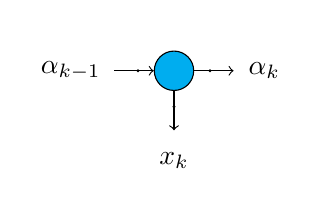
\begin{tikzpicture}[baseline=(G.base), every node/.style={circle, draw, minimum size=5mm}]
  % core box
  \node[fill=cyan] (G) {};
  % left virtual leg
  \draw[<-] (G.west) -- ++(-0.5,0) node[left, draw=none] {$\alpha_{k-1}$};
  % right virtual leg
  \draw[->] (G.east) -- ++(0.5,0) node[right, draw=none] {$\alpha_{k}$};
  % physical leg (down)
  \draw[->] (G.south) -- ++(0,-0.5) node[below, draw=none] {$x_k$};
  % optional small dots to indicate indices
  \fill (G.west) ++(-0.2,0) circle (0.6pt);
  \fill (G.east) ++(0.2,0) circle (0.6pt);
  \fill (G.south) ++(0,-0.2) circle (0.6pt);
\end{tikzpicture}.}}
\]

By convention, we put the flux on the $1$-st TT-core, on the first virtual index of $G^{(1)}$. Thus, the example TT, which encodes the probability distribution for the problem with 4 binary variables, is:

\begin{center}
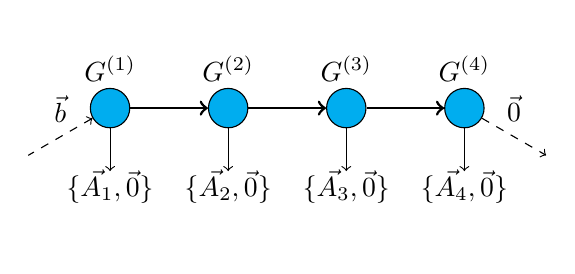
\begin{tikzpicture}[every node/.style={circle, draw, minimum size=5mm}]
    \node[fill=cyan] (x1) at (-2.25, -5) {};
    \node[fill=cyan] (x2) at (-0.75, -5){};
    \node[fill=cyan] (x3) at (0.75, -5) {};
    \node[fill=cyan] (x4) at (2.25, -5) {};

    \node[fill=none, draw=none] (x1_) at (-2.25, -4.5) {$G^{(1)}$};
    \node[fill=none, draw=none] (x2_) at (-0.75, -4.5) {$G^{(2)}$};
    \node[fill=none, draw=none] (x3_) at (0.75, -4.5) {$G^{(3)}$};
    \node[fill=none, draw=none] (x4_) at (2.25, -4.5) {$G^{(4)}$};

    \node[fill=none, draw=none] (c1_) at (-2.25, -6) {$\{\vec{A_1}, \vec{0}\}$};
    \node[fill=none, draw=none] (c2_) at (-0.75, -6) {$\{\vec{A_2}, \vec{0}\}$};
    \node[fill=none, draw=none] (c3_) at (0.75, -6) {$\{\vec{A_3}, \vec{0}\}$};
    \node[fill=none, draw=none] (c4_) at (2.25, -6) {$\{\vec{A_4}, \vec{0}\}$};

    \draw[draw=black, line width=1pt, ->] (x1) -- (x2);
    \draw[draw=black, line width=1pt, ->] (x2) -- (x3);
    \draw[draw=black, line width=1pt, ->] (x3) -- (x4);

    \draw[->] (x1) -- ++(-90:0.8cm);
    \draw[->] (x2) -- ++(-90:0.8cm);
    \draw[->] (x3) -- ++(-90:0.8cm);
    \draw[->] (x4) -- ++(-90:0.8cm);

    \draw[<-, dashed] (x1) -- node[midway, above, pos=0.5, draw=none, fill=none] {$\vec{b}$} ++(-150:1.2cm);
    \draw[->, dashed] (x4) -- node[midway, above, pos=0.5, draw=none, fill=none] {$\vec{0}$} ++(-30:1.2cm);
\end{tikzpicture}.
\end{center}
The charge conservation law \eqref{eq:charge_conservation} is then equivalent to constraints in \eqref{eq:problem_statement}, because it says, that $P(x) \neq 0$ only if $\vec{b}-x_1\vec{A_1}-x_2\vec{A_2}-x_3\vec{A_3}-x_4\vec{A_4}=\vec{0}$.

Building on an exact symmetric TT for the problem \eqref{eq:problem_statement} may be exponentially hard, because it requires an exponentially large number of link charges (thus, exponentially large rank of tensor train). In \cite{LopezPiqueres2023}, heuristic strategies are suggested, which limit the minimum required rank to construct a symmetric tensor train, but also build only the approximation of the required tensor. We describe \textit{Method (i)} in \cref{app:sec:method1}. We chose \textit{Method (ii)} (the most expressive) for this paper as the baseline:

    \textit{Method (ii)}: Given the feasible dataset $\mathcal{T}$, for each $x\in \mathcal{T}$, we calculate all the link charges $c_{\alpha_k}$ by propagating: $c_{1} = \vec{b}$, $c_{\alpha_{i}} = c_{\alpha_{i-1}}-x_i\vec{A_i}$. It requires $|b||\mathcal{T}| (N-1)$ operations, where $|\mathcal{T}|$ is the number of (unique) feasible samples, and $|b|$ is the number of equalities in the problem. Then, for each $G^{(k)}$, we search for consistent (with the left link charges $c_{\alpha_{k-1}}$ and right link charges $c_{\alpha_k}$) site charges $c_{x_k} \in \{\vec{0}, \vec{A_k}\}$. This step requires checking for all $c_{\alpha_{k-1}}$ and $c_{x_k}$, if $(c_{\alpha_{k-1}}-c_{x_k}) \in \bigcup_{\alpha_k}\{c_{\alpha_k}\}$. We store $\bigcup_{\alpha_k}\{c_{\alpha_k}\}$ as a hash-table based type, thus all the checks take $O(N|b||\mathcal{T}|)$ operations on average, and $O(N|b||\mathcal{T}|^2)$ in the worst case (many hash collisions). TT-rank grows with the dataset size as $O(|\mathcal{T}|)$.
    
The process of building a nonzero subspace of the tensor train may be interpreted as building a directed acyclic \textit{charge graph}, with nodes corresponding to link charges, edges corresponding to values of $x_i$, and paths in this graph from the initial node $\vec{b}$ to the final node $\vec{0}$ corresponding to feasible solutions to $Ax=b$. For instance, look at the \cref{fig:example_graph} (a). In these terms, the algorithm of encoding constraints in $U(1)$-symmetric TT is expressive if it generates many feasible paths in the charge graph.

\begin{figure}
\begin{center}
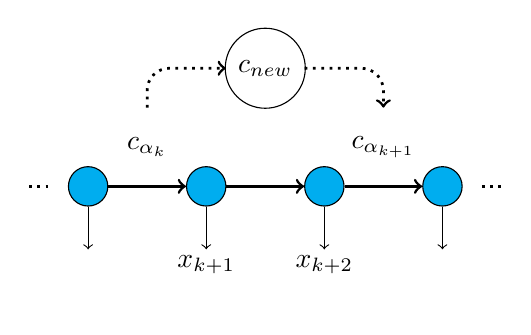
\begin{tikzpicture}[scale=1.0, every node/.style={circle, draw, minimum size=5mm}]
    \node[fill=cyan] (x1) at (-2.25, -5) {};
    \node[fill=cyan] (x2) at (-0.75, -5){};
    \node[fill=cyan] (x3) at (0.75, -5) {};
    \node[fill=cyan] (x4) at (2.25, -5) {};

    \node[fill=none, draw=none] (x1_) at (-2.25, -4.5) {};
    \node[fill=none, draw=none] (x2_) at (-0.75, -4.5) {};
    \node[fill=none, draw=none] (x3_) at (0.75, -4.5) {};
    \node[fill=none, draw=none] (x4_) at (2.25, -4.5) {};

    \node[fill=none, draw=none] (c2_) at (-0.75, -6) {$x_{k+1}$};
    \node[fill=none, draw=none] (c3_) at (0.75, -6) {$x_{k+2}$};
    
    \draw[draw=black, line width=1pt, ->] (x1) -- (x2);
    \draw[draw=black, line width=1pt, ->] (x2) -- (x3);
    \draw[draw=black, line width=1pt, ->] (x3) -- (x4);

    \draw[->] (x1) -- ++(-90:0.8cm);
    \draw[->] (x2) -- ++(-90:0.8cm);
    \draw[->] (x3) -- ++(-90:0.8cm);
    \draw[->] (x4) -- ++(-90:0.8cm);

     \node[fill=none] (cnew) at (0, -3.5) {$c_{new}$};
     \draw[->, line width=1pt, rounded corners=8pt, dotted]
    (-1.5,-4) -- (-1.5,-3.5) -- (-0.5, -3.5);
    \draw[->, line width=1pt, rounded corners=8pt, dotted]
    (0.5, -3.5) -- (1.5, -3.5) -- (1.5, -4);
    \node[draw=none] (ck) at (-1.5, -4.5) {$c_{\alpha_k}$};
    \node[draw=none] (cknext) at (1.5, -4.5) {$c_{\alpha_{k+1}}$};
    \draw[-, dotted, line width=1pt] (-3, -5)--(-2.75, -5);
    \draw[-, dotted, line width=1pt] (2.75, -5)--(3, -5);
    
\end{tikzpicture}
\caption{One step of the EELS algorithm for $\gamma=1$.}
\label{fig:enhancement_scheme}
\end{center}
\end{figure}

\begin{figure*}[h]
\centering
% \begin{tikzpicture}[every node/.style={circle, draw, minimum size=8mm}]
\begin{tikzpicture}[scale=1.0, every node/.style={transform shape, circle, draw, minimum size=8mm}]

    \node[fill=none, draw=none] (a) at (-4, 3) {$a)$};
    \node[fill=none, draw=none] (b) at (-4, -4) {$b)$};
    \node[fill=none, draw=none] (c) at (5.5, 3) {$c)$};
    \node[fill=none, draw=none] (d) at (5.5, -4) {$d)$};
    
    % Upper line (5 circles)
    \node[line width=1pt] (t1) at (-4, 0) {$2$};
    \node[line width=1pt] (t2) at (-2, 2) {$1$};
    \node[line width=1pt] (t3) at (0, 2) {$0$};
    \node[line width=1pt] (t4) at (2, 2) {$0$};
    \node[line width=1pt] (t5) at (4, 0) {$0$};

    % Middle line
    \node[draw=red, line width=2pt] (m) at (0, 0) {$1$};

    % Low line (3 circles)
    \node[line width=1pt] (b1) at (-2, -2) {$2$};
    \node[line width=1pt] (b2) at (0, -2) {$2$};
    \node[line width=1pt] (b3) at (2, -2) {$1$};

    \draw[draw=cyan, line width=1pt, ->] (t1) -- node[midway, above, pos=0.2, draw=none, fill=none] {$x_1=1$}  (t2);
    \draw[draw=cyan, line width=1pt, ->] (t2) -- node[midway, above, draw=none, fill=none] {$x_2=1$} (t3);
    \draw[draw=cyan, line width=1pt, ->] (t3) -- node[midway, above, draw=none, fill=none] {$x_3=0$}(t4);
    \draw[draw=cyan, line width=1pt, ->] (t4) -- node[midway, above, draw=none, fill=none, pos=0.8] {$x_4=0$}(t5);

    \draw[draw=cyan, line width=1pt, ->] (t1) -- node[midway, below, pos=0.2, draw=none, fill=none] {$x_1=0$}(b1);
    \draw[draw=cyan, line width=1pt, ->] (b1) -- node[midway, below, draw=none, fill=none] {$x_2=0$}(b2);
    \draw[draw=cyan, line width=1pt, ->] (b2) -- node[midway, below, draw=none, fill=none] {$x_3=1$}(b3);
    \draw[draw=cyan, line width=1pt, ->] (b3) -- node[midway, below, draw=none, fill=none, pos=0.8] {$x_4=1$}(t5);

    \draw[draw=ForestGreen!70!white, line width=1pt, ->] (t2) -- (m);
    \draw[draw=ForestGreen!70!white, line width=1pt, ->] (m) -- (b3);
    \draw[draw=Yellow!70!white, line width=1pt, ->] (b1) -- (m);
    \draw[draw=Yellow!70!white, line width=1pt, ->](m) -- (t4);


    \node[fill=cyan] (x1) at (-3, -5) {};
    \node[fill=cyan] (x2) at (-1, -5) {};
    \node[fill=cyan] (x3) at (1, -5) {};
    \node[fill=cyan] (x4) at (3, -5) {};

    \node[fill=none, draw=none] (x1_) at (-3, -6.5) {$x_1$};
    \node[fill=none, draw=none] (x2_) at (-1, -6.5) {$x_2$};
    \node[fill=none, draw=none] (x3_) at (1, -6.5) {$x_3$};
    \node[fill=none, draw=none] (x4_) at (3, -6.5) {$x_4$};

    \draw[draw=black, line width=1pt, ->] (x1) -- 
    node[midway, above, pos=0.5, draw=none, fill=none] {$\{1, 2\}$}  
    (x2);
    \draw[draw=black, line width=1pt, ->] (x2) -- 
    node[midway, above, pos=0.5, draw=none, fill=none] {$\{0, \textcolor{red}{1}, 2\}$}  
    (x3);
    \draw[draw=black, line width=1pt, ->] (x3) -- 
    node[midway, above, pos=0.5, draw=none, fill=none] {$\{0, 1\}$}  
    (x4);

    \draw[->] (x1) -- ++(-90:1.2cm);
    \draw[->] (x2) -- ++(-90:1.2cm);
    \draw[->] (x3) -- ++(-90:1.2cm);
    \draw[->] (x4) -- ++(-90:1.2cm);

    \draw[<-, dashed] (x1) -- node[midway, above, pos=0.5, draw=none, fill=none] {$\{2\}$} ++(-150:1.5cm);
    \draw[->, dashed] (x4) -- node[midway, above, pos=0.5, draw=none, fill=none] {$\{0\}$} ++(-30:1.5cm);

    % Equations:
    \node[anchor=west, fill=none, draw=none] at (6,2) {$x_1 + x_2 + x_3 + x_4 = 2$};
    \node[anchor=west, fill=none, draw=none] at (6, 1.2) {$x_i \in \{0, 1\},\quad i = 1\dots4$};
    \node[anchor=west, fill=none, draw=none] at (5.5,-1) {\(
\mathcal{T} = \left[
\begin{array}{c|c}
\textcolor{cyan}{1} & \textcolor{cyan}{0} \\
\textcolor{cyan}{1} & \textcolor{cyan}{0} \\
\textcolor{cyan}{0} & \textcolor{cyan}{1} \\
\textcolor{cyan}{0} & \textcolor{cyan}{1}
\end{array}
\right]
\)};

    \node[anchor=west, fill=none, draw=none] at (5.5,-5) {\(
\mathcal{X} = \left[
\begin{array}{c|c|c|c}
\textcolor{cyan}{1} & \textcolor{cyan}{0} & \textcolor{ForestGreen!70!white}{1} & \textcolor{Yellow!70!white}{0} \\
\textcolor{cyan}{1} & \textcolor{cyan}{0} & \textcolor{ForestGreen!70!white}{0} & \textcolor{Yellow!70!white}{1} \\
\textcolor{cyan}{0} & \textcolor{cyan}{1} & \textcolor{ForestGreen!70!white}{0} & \textcolor{Yellow!70!white}{1}\\
\textcolor{cyan}{0} & \textcolor{cyan}{1} & \textcolor{ForestGreen!70!white}{1} & \textcolor{Yellow!70!white}{0}
\end{array}
\right]
\)};
\end{tikzpicture}
\caption{Example problem, where EELS reveals new samples, while standard approaches do not find any new feasible solutions. a) Charge graph of the problem. Cyan paths correspond to the training data, green and yellow lines show new feasible samples after local search. Red charge is a "newborn" charge. b) TT and the link charges nodes, obtained from the training data (black) and found by local search (red). c) Problem constraints and initial feasible dataset. d) All possible unique samples. The sample color in $\mathcal{X}$ matches the color of the corresponding path in the graph.}
\label{fig:example_graph}
\end{figure*}

\subsection{Expressibility Enhancement Local Search (EELS)}
\label{subsec:eels}
We noticed that all methods for building symmetric TT from data, as suggested in \cite{LopezPiqueres2023}, may fail for the same reason. Methods take link charges only from the data but do not apply any strategy to search for unknown charges. If the training data is too small or not diverse enough, then the required link charges, which encode near-optimal solutions, simply do not appear in TT. Moreover, this disadvantage may not be compensated during the training step, because the charge structure pre-defines all samples, which may be sampled from symmetric TT \textit{in principle}, and the learning procedure updates only the probabilities of principally possible samples.

\begin{figure}[h!]
    \centering

    \begin{subfigure}{0.5\textwidth}
        \centering
        
\includegraphics[width=\linewidth]{pictures/assignment_400_merged.pdf}
        \caption{$\left|T\right|=400$.}
        \label{fig:assignemnt_400_abs}
    \end{subfigure}
    \hspace{10pt}
    
    \begin{subfigure}{0.5\textwidth}
        \centering
        
\includegraphics[width=\linewidth]{pictures/assignment_4000_merged.pdf}
        \caption{$\left|T\right|=4000$.}
        \label{fig:assignment_4000_abs}
    \end{subfigure}
    \hspace{10pt}

    \begin{subfigure}{0.5\textwidth}
        \centering
        
\includegraphics[width=\linewidth]{pictures/assignment_10000_merged.pdf}
        \caption{$\left|T\right|=10000$. }
        \label{fig:assignment_10000_abs}
    \end{subfigure}
    \hspace{10pt}

    \caption{Number of unique samples in TT for different $U(1)$-symmetric TT building strategies on the assignment problem.}
    \label{fig:assignment_experiments}
\end{figure}

\begin{figure*}[h!]
    \centering

    \begin{subfigure}{0.48\textwidth}
        \centering
        
\includegraphics[width=\linewidth]{pictures/Num_samples_r1.pdf}
        \caption{N=50, m=5, r=1.}
        \label{fig:T4_T5}
    \end{subfigure}
    \hspace{10pt}
    \begin{subfigure}{0.48\textwidth}
        \centering
        
\includegraphics[width=\linewidth]{pictures/Time_r1.pdf}
        \caption{N=50, m=5, r=1.}
        \label{fig:num_samples_time}
    \end{subfigure}
    \hspace{10pt}
    \begin{subfigure}{0.48\textwidth}
        \centering
        \includegraphics[width=\linewidth]{pictures/Num_samples_sparse_r1_relative.pdf}
        \caption{N=75, m=5,10; r=1.}
        \label{fig:random_r1_rel}
    \end{subfigure}
    \hspace{10pt}
    \begin{subfigure}{0.48\textwidth}
        \centering
        
\includegraphics[width=\linewidth]{pictures/Num_samples_sparse_r2_relative.pdf}
        \caption{N=75, m=5,10; r=2.}
        \label{fig:random_r2_rel}
    \end{subfigure}
    % \hfill

    \caption{Comparison of $U(1)$-symmetric TT building strategies on random problems with $N$ binary variables, $m$ linear equalities and constraints matrix sampled from uniform distribution in range $ [-r, r] $. (a) Number of samples dependency on training dataset size. (b) Wall time to build initial $U(1)$-symmetric TT. (c),(d) Num sumpes ratio on matrix sparsity.}
    \label{fig:num_samples_random}
\end{figure*}

For example, look at the combinatorial problem and dataset $\mathcal{T}$ on \cref{fig:example_graph} (c). Method (ii) fails to find any new samples that do not appear in $\mathcal{T}$. On \cref{fig:example_graph} (a), black circles are the link charges obtained from $\mathcal{T}$, and cyan arrows are all paths in the graph, which encode the dataset samples. Obviously, no new path exists through the black charges, which satisfy the charge conservation law $c_{\alpha_{k+1}} = c_{\alpha_k} - x_{k+1}$ on each edge; thus, no new samples were obtained in TT. 

We propose a new parameterized family of methods for initializing symmetric TT, called Expressibility Enhancement Local Search (EELS). First, we initialize symmetric TT with Method (ii). Then, we apply the expressibility enhancement phase. The \cref{fig:enhancement_scheme} illustrates the main idea of this phase: we fix the $k$-th link of TT, and then search for such charges $c_{new}$, which i) do not appear at the $k+1$-th link; ii) may connect the charges at the $k$-th link with the charges at the $(k+2)$-th link, satisfying charge conservation law for some $x_{k+1}$, $x_{k+2}$. Thus, we "jump" over the $k+1$-th link, and conduct a local search in a charge graph, finding such $c_{\alpha_{k}}$, $x_{k+1}$, $x_{k+2}$, which satisfy the $U(1)$-symmetry. Sometimes this procedure spawns new charges, which may be assigned to the $k+1$-th link. The length of the "jump" may be regulated with the parameter $\gamma$, which is equal to the number of links we jump over. At the \cref{fig:enhancement_scheme}, $\gamma=1$, and the \cref{alg:enhance_expressibility} also provides the detailed description for $\gamma=1$. Method (ii) may be associated with $\gamma=0$. For $\gamma>1$, we search for new charges at the links $k+1$, $k+2$, ..., $k+\gamma$ simultaneously, by considering all possible combinations of $c_{\alpha_k}$, $x_{k+1}$, ..., $x_{k+\gamma + 1}$, thus, the complexity of the algorithm is $O\left(2^{\gamma + 1}|\mathcal{T}| |b|(N-\gamma)\right)$ on average. \cref{fig:example_graph} shows that even for $\gamma=1$, our expressibility enhancement procedure may find some new charges, and thus, new paths in the charge graph, corresponding to feasible samples.


\begin{algorithm}
\caption{EELS algotithm, $\gamma=1$}
\label{alg:enhance_expressibility}
\begin{algorithmic}[1]

\REQUIRE $C_1,\dots, C_{N-1}$  - Sets of link charges, defined from data; $A, b$ - constraints for the problem; $G^{(1)}, \dots ,G^{(N)}$ - TT-cores;

\STATE $c_{\alpha_0}\gets \vec{b}$, $c_{\alpha_N} \gets \vec{0}$

\FOR{$k = 1$ \textbf{to} $N - 2$}
    \FOR{$c_{\alpha_k} \in C_k$}
        \FOR{$x_{k+1} \in \{0, 1\}$}
            \STATE $c_{new} \gets c_{\alpha_k} - x_{k+1}\vec{A_{k+1}}$
            \FOR{$x_{k+2} \in \{0, 1\}$}
                \IF {$c_{new} - x_{k+2}\vec{A_{k+2}} \in C_{k+2}$}
                    \STATE $c_{\alpha_{k+2}} = c_{new} - x_{k+2}\vec{A_{k+2}}$
                    \STATE $C_{k+1}$.add($c_{new}$)
                    \STATE Insert new nonzero blocks:
                    \STATE $G^{(k+1)}\gets (c_{\alpha_{k}}, x_{k+1}\vec{A_{k+1}}, c_{new})$
                    \STATE $G^{(k+2)}\gets (c_{new}, x_{k+2}\vec{A_{k+2}},c_{\alpha_{k+2}})$
                \ENDIF
            \ENDFOR
        \ENDFOR
    \ENDFOR
\ENDFOR
\end{algorithmic}
\end{algorithm}

We emphasize that EELS has nothing in common with regular local search, which may be applied to the data samples to obtain new solution candidates. It acts more like a crossover operator, entangling all the samples from $\mathcal{T}$. On \cref{fig:example_graph}(a), EELS obtains the solution, which takes the first bit of the solution $1100$, and the last bit from the solution $0011$, and the bits $00$ in the middle are found using the charge conservation law. Similarly, EELS also finds a feasible solution, taking the first bit from $0011$ and the last bit from $1100$, filling the middle with a guess of $11$. For large datasets, EELS may generate new feasible candidates by mixing all samples from $\mathcal{T}$, producing unpredictable bit concatenations with some "guessed" fillers. 

\subsection{Amplification of Data Diversity (ADD)}
\label{subsec:add}

EELS from \cref{subsec:eels} is useful when we lack training data or want to better exploit existing data. In this section, we consider the special case of constraints $Ax=b$ when a feasible dataset sampler is available, or it is easy to construct a large dataset $\mathcal{T}$ using extra knowledge. Such situations include, for instance, cardinality constraints $\sum_{i=1}^N x_i=\kappa$. In this case, because tensor train optimization trains on the fly, we probably should not use the entire available data but rather pick a good, diverse subset. Otherwise, the complexity of the training step may be (too) large.

We formulate a problem as follows. Let $\mathcal{T}$ be a data, available at the $t$-th iteration of the \cref{alg:tt_generative}. This data includes samples from TT and other feasible solutions generated by the feasible data sampler. How to choose a subset $\mathcal{T}'\subset \mathcal{T}$, such that $|\mathcal{T}'| = \mu < |\mathcal{T}|$, to achieve exploration-exploitation trade-off, and keep the complexity of the training step manageable? We need to define the measure of the sample's novelty relative to what the generative scheme has already explored. To do this, we give a formal definition of the charge graph for the problem \eqref{eq:problem_statement}, which we discuss informally in \cref{subsec:eels}.
Let $|b|=m$ be the number of equalities in problem \eqref{eq:problem_statement} and $N$ the number of binary variables. Let consider a DAG $D=(V, E, \omega, \xi)$, with $\omega: V\to \mathbb{R}^m$ and $\xi: E \to \{\{0\}, \{1\}, \{0,1 \}\}$. Here $\omega(v)$ is a charge of the vertex $v$, and the set of all vertices consists of several layers: $V = L_0 \sqcup L_1 \sqcup \dots \sqcup L_N.$
We call such a graph a charge graph of problem \eqref{eq:problem_statement} if all of the following stand:

\begin{enumerate}
    \item $|L_0| = |L_N| = 1$, $\omega(v_0\in L_0) = \vec{b}$, $\omega(v_N\in L_N)=\vec{0}$
    \item $(u, v) \in E \Rightarrow u\in L_i, \: v \in L_{i+1}$ for some $i$ 
    \item If $u_k\in L_k$, and $v_{k+1}\in L_{k+1}$, then $\omega(u_k)-\omega(v_{k+1})=\vec{0}$ or $\omega(u_k)-\omega(v_{k+1})=\vec{A_{k+1}}$, where $\vec{A_{k+1}}$ is a $k$-th column of the matrix $A$
    \item $\xi(e(u_k, v_{k+1})) = \{0, 1\}$, if $\vec{A_{k+1}} = \vec{0}$, else $\xi(e(u_k, v_{k+1})) = \{0\}$ if $\omega(u_k)=\omega(v_{k+1})$, or $\xi(e(u_k, v_{k+1})) = \{1\}$ if $\omega(u_k)-\omega(v_{k+1})=\vec{A_{k+1}}$.
\end{enumerate}

Charge graph on \cref{fig:example_graph}(a) satisfies all conditions from the definition. On each path $p$ with edges $(e_1, \dots e_N)$ from $v_0 \in L_0$ to $v_N \in L_N$, we define the operation of feasible subset evaluation: $F(p) = \xi(e_1) \times \dots \times \xi(e_N)$, where "$\times$" is the Cartesian product. We call a charge graph \textit{full} if the set $\mathcal{F}(D)=\bigsqcup_{p\in \mathcal{P}(\mathcal{D})}F(p)$ coincides with all the solutions of $Ax=b$, where $\mathcal{P}(\mathcal{D})$ is a set of all the paths from $v_0$ to $v_N$. We define the width of the charge graph as $|D|=\max_{k=0}^{N}\left(|L_k|\right)$. 

The search for the full graph charge may be exponentially hard, and the same is true for storing such a graph. That is why Method (ii) from \cref{subsec:U1_generative} builds only a subgraph $H\subset D$ with a limited width $|H|\leq |\mathcal{T}|$. The goal of the $U(1)$-generative approach is to find such $H\subset D$, that $x^{*} \in \mathcal{F}(H)$ for the optimal solution $x^{*}$ of problem \eqref{eq:problem_statement}. The structure of $H$, which is explored on the training step in \cref{alg:tt_generative}, is completely defined by the selection of samples from the whole available samples set $\mathcal{T_\text{new}}\subset S$. The articles \cite{Alcazar2024} and \cite{LopezPiqueres2023} suggest only the selection of samples with the best cost function $C(x)$, or picking up some rare samples from $S$ for diversity. We suggest using graph distance as a diversity measure. Let $\mathcal{S}=(V^{\mathcal{S}}, E^{\mathcal{S}}, \omega^{\mathcal{S}}, \xi^{\mathcal{S}})$ be a charge graph for some feasible solution $s=(x_1,\dots, x_N)$. Let $V^{\mathcal{S}}=\bigsqcup_k \{v_k\}$. On each step of the generative optimization, we store a charge graph of already seen samples $\mathcal{H}$, as the sets of charges for each vertex layer: $C_k^{\mathcal{H}} = \bigsqcup_{v\in L_k^{\mathcal{H}}} \{\omega_{\mathcal{H}}(v)\}$. Then the graph distance between $\mathcal{S}$ and $\mathcal{H}$ is:

\begin{equation}
    \rho(\mathcal{S}, \mathcal{H}) = \sum_{k=1}^{N-1}\left(1 - \chi(\omega^{\mathcal{S}} (v_k) \in C_k^{\mathcal{H}})\right),
\label{eq:graph_distance}
\end{equation}

where $\chi(\cdot)$ is an indicator function of the condition in brackets. Thus, we count the number of new charges that appear in the solution $s$ and were not previously seen by the algorithm. In \cref{sec:results} we discuss how to balance this novelty measure with exploitation of the near-optimal samples.

\section{Results}
\label{sec:results}

\subsection{Comparison of EELS with other methods}
\label{subsec:eels_res}
We may compare the expressibility of the methods of building $U(1)$-symmetric tensor trains by fixing the dataset $\mathcal{T}$, defining all link charges degeneracy ranks in \eqref{eq:direct_sum} $\dim(V^{(c_k)}) = 1$ and then, calculating the number of nonzero elements. 
If we initialize $G^{(k)}(\alpha_{k-1}, x_k, \alpha_k)= 1$ for all positions, preserving $U(1)$-symmetry, then $\pi(x)=1$ for all $x$, conserving charge $b$. Thus, the number of unique samples in tensor train is just a Frobenius norm squared, which may be calculated efficiently in TT-format.

\cref{fig:num_samples_random} shows the group of experiments for the problem \eqref{eq:problem_statement} with the random matrices $A$ of size $m\times n$ and random vector $b$, both sampled from the uniform distribution on $[-r, r]$. \cref{fig:T4_T5} shows the dependency of the number of unique samples in $U(1)$-symmetric TT as the function of training dataset size. With EELS, the number of unique samples grows as $\sim|\mathcal{T}|^5$ for $r=1$, while applying only the baseline method (Method (ii) from \cref{subsec:U1_generative}) encodes only $\sim|\mathcal{T}|^4$ possible feasible solutions. EELS improves the baseline with a small increase in computational time to build an initial $U(1)$-symmetric TT, as shown in \cref{fig:num_samples_time}. Other experiments on \cref{fig:num_samples_random} demonstrate that the benefit of using EELS depends a lot on the sparsity of the matrix $A$, the number of constraints, and the value of parameter $r$. Generally, if $r$ is big, or the number of constraints is huge, then it is hard to satisfy the if-condition in line 7 of \cref{alg:enhance_expressibility}, and EELS spawns only a small fraction of new link charges $c_{new}$, if it spawns any at all. 
In contrast, if the matrix $A$ is sparse, EELS may be an efficient strategy for several dozen constraints. For example, we consider an assignment problem \cite{koopmans1957assignment}. This is NP-hard problem for a quadratic/black-box oracle  $C(x)$. The constraints matrix of size $2n \times n^2$ is given by the rule:

\begin{equation}
\left\{
\begin{aligned}
    & A_{j, (i-1)n+j} = 1, \quad \forall i,j = 1, \dots, n\\[4pt]
    & A_{n+i, (i-1)n+j} = 1, \quad \forall i,j = 1, \dots, n\\[4pt]
    & \text{else} \quad A_{k, m} = 0,
\end{aligned}
\right.
\label{eq:assignment_matrix}
\end{equation}
and $b_i=1 \quad \forall i = 1, \dots ,2n$. The density of matrix $A$ scales as $O(\frac{1}{n})$. \cref{fig:assignment_experiments} shows the group of experiments with the assignment problem. 
The total number of feasible samples grows monotonically with the problem size as $n!$; however, for large problems, building symmetric  TT methods struggle to find new feasible samples when the training data is insufficiently expressive. That is why the number of samples in TT saturates and then decreases. The peak of saturation shifts to the right as the initial dataset size grows. EELS provides approximately $3-6$ times more samples at the peak point than Method (ii) from \cref{subsec:U1_generative}.

\subsection {ADD impact on optimization results}
\label{subsec:diversify_data_res}
% \begin{itemize}
%     \item Description of each strategy: best cost, mixed, weighted rank, best cost (+ nonzero graph distance), complexity of each strategy, complexity of graph distance;
%     \item Num wins/losses for different selection strategies;
% \end{itemize}

We use the graph distance \cref{eq:graph_distance} to balance the novelty of the samples and the exploitation of near-optimal samples on the data selection step 4 of \cref{alg:tt_generative}. The assignment problem gives exactly the setting described in \cref{subsec:add}: all feasible samples can be generated from permutations of $n$ elements. Thus, it is not a problem to obtain the dataset of feasible samples $\mathcal{T}$, but to choose which data is worth learning. In our experiments, we sample $K/2$ candidates for the dataset $S$ from $P_{\theta}$, and $K/2$ candidates from the random feasible sampler, and limit the number of samples used for training to $\mu$, because training is an expensive procedure. For some strategies, we also store the graph of all already seen charges $\mathcal{H}$, as a set of charges for each TT link index $i$. The computation of $\rho(\mathcal{S}, \mathcal{H})$ is then requires $O(|b|(N-1))$ operation in average, and storing $\mathcal{H}$ produces extra memory overhead. In our experiments, these parts were not the bottleneck of the whole algorithm; the most intensive step is training, which includes gradient evaluation, sparse core updates, and, for 2-site DMRG, also concatenations and reshapes with $U(1)$-tensors.
We suggest three strategies of data selection, and compared them with the baseline from \cite{LopezPiqueres2023}:

\begin{enumerate}
    \item \textit{Best Cost} (Baseline): Pick data from $\mathcal{T_{\text{new}}} \subset S$ with the best cost function $C(s)$ values. 
    \item \textit{Best Cost + Graph Distance Filter}: Pick $(1-w_{filter})\mu$ samples from $\mathcal{T_{\text{new}}} \subset S$ with the best cost function $C(s)$, then filter remaining data based on condition $\rho(\mathcal{S}, \mathcal{H}) > 0$ and take $w_{filter} \mu$ samples with the best cost. The filtering with $0 < w_{filter} \leq 1$ ensures that any new data that in $S$ will be used for training.
    \item \textit{Mixed Selection}: Pick $(1-w_{mix})\mu$ samples from $S$ based on the best cost, and $w_{mix}\mu$ samples based on the largest values of graph distance $\rho(\mathcal{S}, \mathcal{H})$, $0 < w_{mix} \leq 1$. This strategy picks the "newest" samples, maximizing diversity of the training data.
    \item \textit{Weighted Rank}: Pick samples from $S$ based on the lowest weighted rank sum $r_C + w_{rank}r_{\rho}$, where $r_C$ is a rank of sample based on cost function value ($r_C=1$ for $s$ with the minimal $C(s)$) and $r_{\rho}$ is a rank of the sample based on graph distance ($r_{\rho} = 1$ for the sample $s$ with the maximal $\rho(\mathcal{S}, \mathcal{H})$), $0< w_{rank} < +\infty$.
\end{enumerate}

\begin{figure}
    \centering
    \includegraphics[width=0.5\textwidth]{pictures/LibsComparison.pdf}
    \caption{Wall time for assignment problem. Each algorithm performs one iteration, with one sweep, and the training data size is $|T|=400$.
    The degeneracy of the block $\dim(V^{(c_k)}) = 1$ for each link index.}
    \label{fig:lib_comparison}
\end{figure}

The corrected-gradient exploratory comparison does not show uniform dominance of all diversity-aware strategies over the Best Cost baseline. Their performance depends on the selection rule, its weight $w$, and the objective-function family. The complete exploratory results used for strategy and hyperparameter selection are reported in \cref{app:selection_strategy_screening}, including \cref{fig:SelectionStrategiesVOne,tab:selection_strategy_screening}. We therefore use these results only for model selection and do not interpret the largest observed improvement as a confirmatory effect estimate.

After fixing the best-performing strategy and its weight using the exploratory experiments, we evaluated this single configuration against Best Cost on an independent set of previously unseen assignment problems. The held-out A/B results are shown in \cref{fig:independent_ab_tests}; the corresponding paired-test statistics should be reported separately for the linear and quadratic objectives in \cref{tab:independent_ab_tests}. Wins denote instances on which the selected strategy obtains a lower final cost than Best Cost, losses denote the converse, and ties denote equal final costs.

\begin{figure*}[t]
    \centering
    \begin{subfigure}{0.48\textwidth}
        \centering
        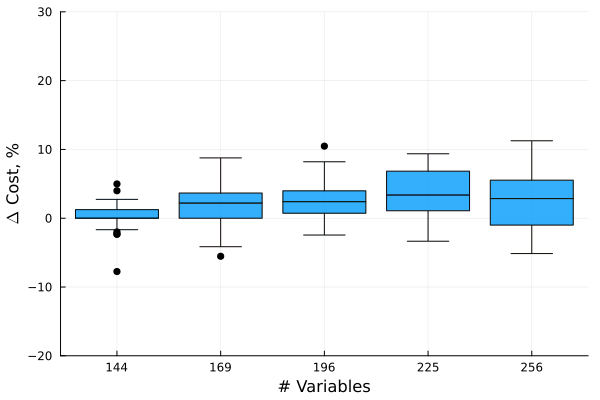
\includegraphics[width=\linewidth]{examples/pictures/test_Linear.png}
        \caption{Linear objective, $c^T x$.}
        \label{fig:independent_ab_linear}
    \end{subfigure}
    \hfill
    \begin{subfigure}{0.48\textwidth}
        \centering
        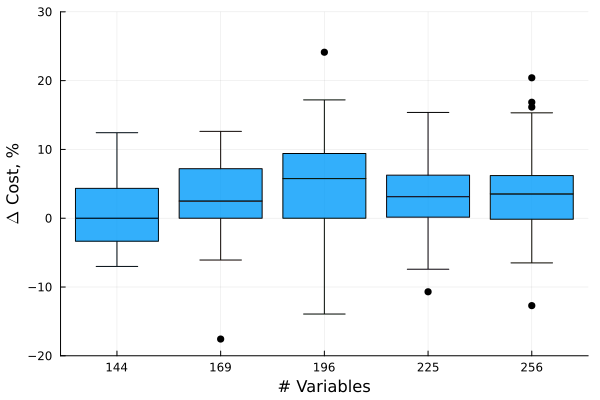
\includegraphics[width=\linewidth]{examples/pictures/test_Quadratic.png}
        \caption{Quadratic objective, $x^TQx$.}
        \label{fig:independent_ab_quadratic}
    \end{subfigure}
    \caption{Confirmatory A/B evaluation of the selected diversity-aware strategy against the Best Cost baseline on independent held-out problem instances. Strategy selection and tuning of $w$ were completed before evaluating these data.}
    \label{fig:independent_ab_tests}
\end{figure*}

\begin{table*}[t]
    \centering
    \caption{Confirmatory paired comparison on independent held-out data. Replace \texttt{TBD} with the final results. The $p$-value is from the pre-specified paired test, and the effect size is the relative improvement over Best Cost.}
    \label{tab:independent_ab_tests}
    \begin{tabular}{llrrrrrr}
        \toprule
        Objective & Selected strategy & $w$ & Wins & Losses & Ties & $p$-value & Effect (\%) \\
        \midrule
        Linear, $c^T x$ & \texttt{TBD} & \texttt{TBD} & \texttt{TBD} & \texttt{TBD} & \texttt{TBD} & \texttt{TBD} & \texttt{TBD} \\
        Quadratic, $x^TQx$ & \texttt{TBD} & \texttt{TBD} & \texttt{TBD} & \texttt{TBD} & \texttt{TBD} & \texttt{TBD} & \texttt{TBD} \\
        \bottomrule
    \end{tabular}
\end{table*}

\subsection{Benchmarking library performance}
\label{subsection: bench_perf_res}

The implementation of \cite{LopezPiqueres2023} is not open-source. However, the more recent article by the same authors has a GitHub repo \texttt{ConstrainTNet} \cite{ConstrainTNet2024}. It implements exact approach to building $U(1)$-symmetric TT (no data is needed for initialization, but initialization may be computationally intractable for difficult constraints). Nevertheless, \cite{ConstrainTNet2024} also uses \texttt{iTensors} \cite{ITensor} dependency. We compared the libraries performance on the assignment problem, excluding the time to build symmetric TT from both methods, since it is done in a fundamentally different way. However, the training and sampling strategies coincide and can be compared directly based on runtime for the same initial tensor. Results are provided on \cref{fig:lib_comparison}. 
It seems that our library is $\times 100$ faster (we do not use \texttt{iTensors} and rely on our own back-end implemented in \texttt{Julia}). We tested the script from the example folder of the \texttt{ConstrainTNet} git \cite{ConstrainTNetQuadraticKnapsack2024} (with $A$ and $b$ for the assignment problem) and measured the wall time. The result may be the consequence of our optimizations, aimed at speeding up the computations in a non-degenerate case, with more than a dozen constraints (while \texttt{iTensors} aims at more general tensor computations). All our code is available at git \cite{OhMyU1_2026}.

\section{Acknowledgements}
We thank Margarita Veshchezerova for providing the initial impetus for this research. We are grateful to Dmitry Gribanov, Elizaveta Iarovikova, Maxim Klimenko, and Ivan Samoylenko for insightful discussions. We appreciate the anonymous reviewers for their helpful feedback.

\section{Impact Statement}
This work advances methods for black-box constrained combinatorial optimization by leveraging a low-rank symmetric tensor decomposition within the generative Machine Learning approach. The scope of potential applications includes all problems where the cost function structure is unknown and some hard linear constraints must be satisfied. As a result, practitioners in logistics, scheduling, resource allocation, engineering design, and scientific simulation can obtain better solutions faster, lowering computational budgets and accelerating iteration cycles in real‑world workflows. We aim to make these benefits accessible: the paper documents algorithms, provides reproducibility artifacts \cite{OhMyU1_2026}.

\bibliography{refs}
\bibliographystyle{icml2026}

\newpage
\appendix
\onecolumn

\section{TT Generative Modeling implementation details}
\label{app:sec:implement_vars}
In \cref{alg:tt_generative}, if the objective function $C(x)$ is computationally expensive, only a fraction of samples may be evaluated, and the remaining samples are assigned probability weights heuristically. The probability distribution for the samples may be replaced with another physically motivated distribution, such as the Fermi-Dirac distribution. For minimizing $\mathcal{L}(\theta)$, usually the Density Matrix Renormalization Group (DMRG) algorithm is used, which optimizes each TT-core alternatingly \eqref{eq:tt-def}, or optimizes merged TT-cores (2-site DMRG variation). An optional annealing schedule may gradually decrease the temperature parameter to sharpen the distribution around low-cost regions. 

\section{Strategies of building $U(1)$-symmetric TT}
\label{app:sec:method1}

\textit{Method (i)}: Given the feasible dataset $\mathcal{T}$, for each $x\in \mathcal{T}$, we calculate all the link charges $c_{\alpha_k}$ by propagating: $c_{1} = \vec{b}$, $c_{\alpha_{i}} = c_{\alpha_{i-1}}-x_i\vec{A_i}$. It requires $|b||\mathcal{T}| (N-1)$ operations, where $|\mathcal{T}|$ is the number of (unique) feasible samples, and $|b|$ is the number of equalities in the problem. Then, we initialize each TT-core $G^{(k)}$ with non-zero blocks for subspace with charges $(c_{\alpha_{k-1}}, x_k \vec{A_k}, c_{\alpha_k})$.

\section{Exploratory comparison of data-selection strategies}
\label{app:selection_strategy_screening}

We used the following experiments to screen the proposed data-selection strategies and choose their weights before the independent evaluation reported in \cref{subsec:diversify_data_res}. Each box is obtained from 50 random assignment problems. The baseline is Best Cost; all other hyperparameters of the generative scheme, including $|\mathcal{T}|=1000$ and $K=2\cdot10^4$, are fixed. For the linear objective, $c$ is sampled uniformly on $[-50,50]$; for the quadratic objective, the entries of $Q$ are sampled uniformly on $[-7,7]$. These exploratory results are not uniformly favorable to every strategy and should not be interpreted as an independent confirmatory test.

\begin{figure*}[h!]
    \centering

    \begin{subfigure}{0.48\textwidth}
        \centering
        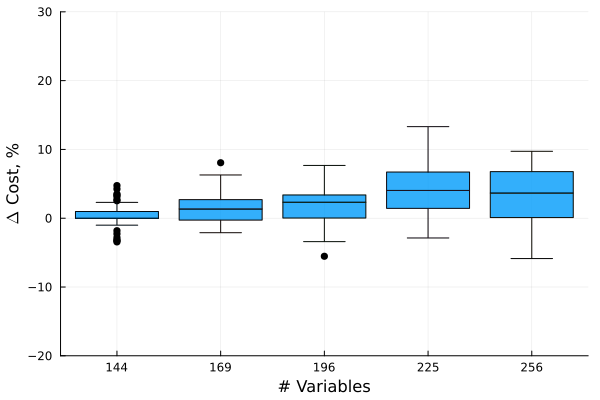
\includegraphics[width=\linewidth]{examples/pictures/BestCost_vs_MixedNonzero_v1.png}
        \caption{Linear: Best Cost + Graph Distance Filter, $w_{\text{filter}}=0.3$.}
        \label{fig:BestCost_vs_MixedNonzeroVOne}
    \end{subfigure}
    \hfill
    \begin{subfigure}{0.48\textwidth}
        \centering
        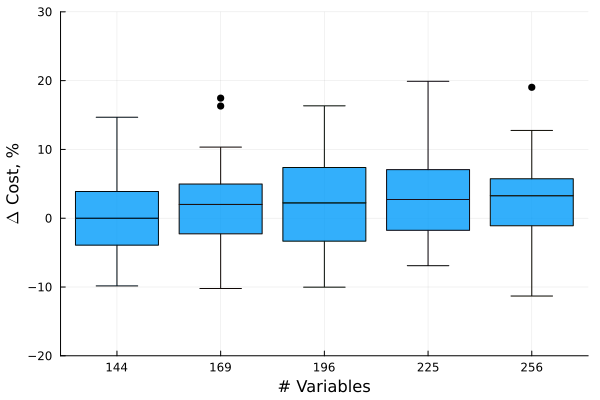
\includegraphics[width=\linewidth]{examples/pictures/BestCost_vs_MixedNonzero_quadratic_v1.png}
        \caption{Quadratic: Best Cost + Graph Distance Filter, $w_{\text{filter}}=0.3$.}
        \label{fig:BestCost_vs_MixedNonzeroQuadraticVOne}
    \end{subfigure}

    \begin{subfigure}{0.48\textwidth}
        \centering
        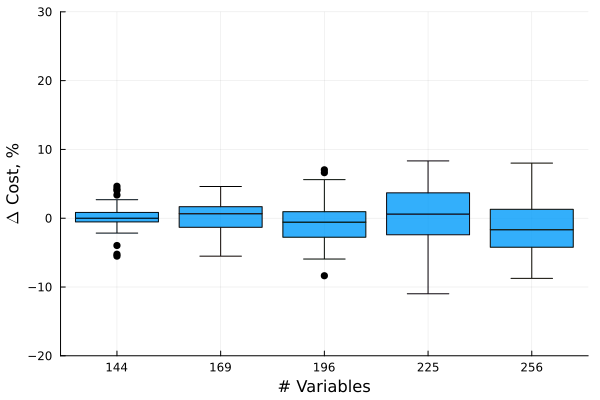
\includegraphics[width=\linewidth]{examples/pictures/BestCost_vs_Mixed_v1.png}
        \caption{Linear: Mixed Selection, $w_{\text{mix}}=0.4$.}
        \label{fig:BestCost_vs_MixedVOne}
    \end{subfigure}
    \hfill
    \begin{subfigure}{0.48\textwidth}
        \centering
        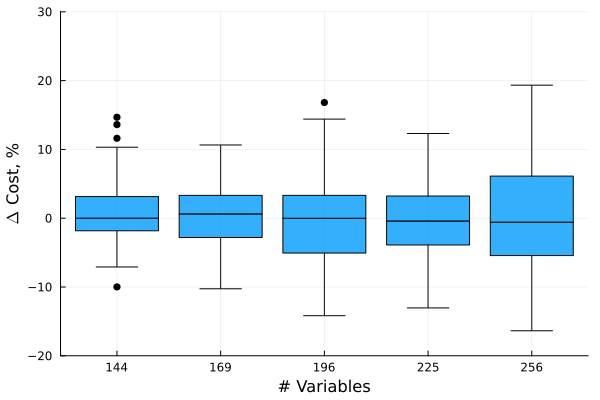
\includegraphics[width=\linewidth]{examples/pictures/BestCost_vs_Mixed_quadratic_v1.png}
        \caption{Quadratic: Mixed Selection, $w_{\text{mix}}=0.4$.}
        \label{fig:BestCost_vs_MixedQuadraticVOne}
    \end{subfigure}

    \begin{subfigure}{0.48\textwidth}
        \centering
        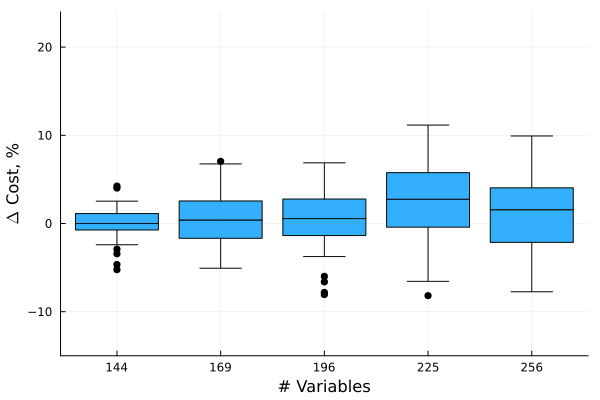
\includegraphics[width=\linewidth]{examples/pictures/BestCost_vs_WeightedRank_v1.png}
        \caption{Linear: Weighted Rank, $w_{\text{rank}}=0.7$.}
        \label{fig:BestCost_vs_WeightedRankVOne}
    \end{subfigure}
    \hfill
    \begin{subfigure}{0.48\textwidth}
        \centering
        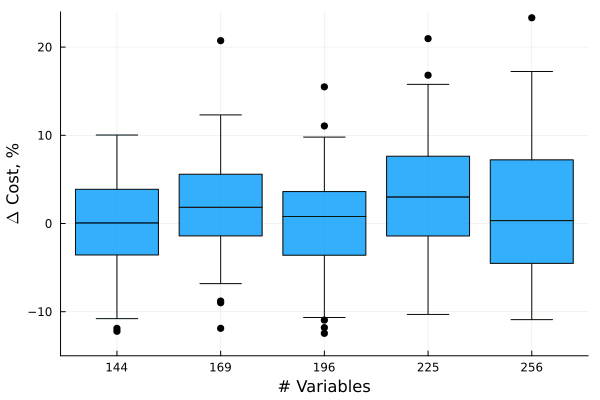
\includegraphics[width=\linewidth]{examples/pictures/BestCost_vs_WeightedRank_quadratic_v1.png}
        \caption{Quadratic: Weighted Rank, $w_{\text{rank}}=0.7$.}
        \label{fig:BestCost_vs_WeightedRankQuadraticVOne}
    \end{subfigure}

    \caption{Exploratory relative cost improvement over the Best Cost baseline after correcting the symmetric-TT gradient. These data were used for strategy and hyperparameter selection.}
    \label{fig:SelectionStrategiesVOne}
\end{figure*}

\begin{table*}[h!]
    \centering
    \caption{Exploratory paired comparisons with Best Cost. Replace \texttt{TBD} with the final counts and effect estimates. Wins denote lower final cost for the named strategy.}
    \label{tab:selection_strategy_screening}
    \begin{tabular}{llrrrrr}
        \toprule
        Objective & Strategy & $w$ & Wins & Losses & Ties & Effect (\%) \\
        \midrule
        Linear & Best Cost + Graph Distance Filter & 0.3 & \texttt{TBD} & \texttt{TBD} & \texttt{TBD} & \texttt{TBD} \\
        Linear & Mixed Selection & 0.4 & \texttt{TBD} & \texttt{TBD} & \texttt{TBD} & \texttt{TBD} \\
        Linear & Weighted Rank & 0.7 & \texttt{TBD} & \texttt{TBD} & \texttt{TBD} & \texttt{TBD} \\
        Quadratic & Best Cost + Graph Distance Filter & 0.3 & \texttt{TBD} & \texttt{TBD} & \texttt{TBD} & \texttt{TBD} \\
        Quadratic & Mixed Selection & 0.4 & \texttt{TBD} & \texttt{TBD} & \texttt{TBD} & \texttt{TBD} \\
        Quadratic & Weighted Rank & 0.7 & \texttt{TBD} & \texttt{TBD} & \texttt{TBD} & \texttt{TBD} \\
        \bottomrule
    \end{tabular}
\end{table*}

\end{document}
